The Form Builder allows users to assign a form to a task and customize its data fields (Figure~\ref{fig:form_builder}).

The forms data fields are displayed in the centre of the screen in a grid layout.
The number of columns of the grid layout can be modified in the right side panel.
The default value is 4 columns.
The minimal number of columns is 2 and maximal is 6.

Data field can be placed in the layout by dragging it from the left side panel where all types of data fields are available.
At the bottom of the list are all fields that exist in the given process.
Existing fields that are already used in the current form are disabled for dragging.

Further customization of data field style is possible by creating a custom field by clicking the fast action button on the right border of the left side panel.
A dialog is then opened where the user has to select the fields type and title and insert the custom HTML and CSS\@.
After clicking the Save button the new field is added to the list in the left side panel and ready to use.

Data field can be selected by clicking on it.
Settings of the selected data field are shown in the right side panel where you can edit the following properties:
\begin{itemize}
  \item behavior,
  \item netgrif template,
  \item style,
  \item label,
  \item placeholder,
  \item description,
  \item value,
  \item options (only available for enumeration and multichoice fields).
\end{itemize}
Any change is automatically saved.

\begin{figure}[h!]
  \centering
  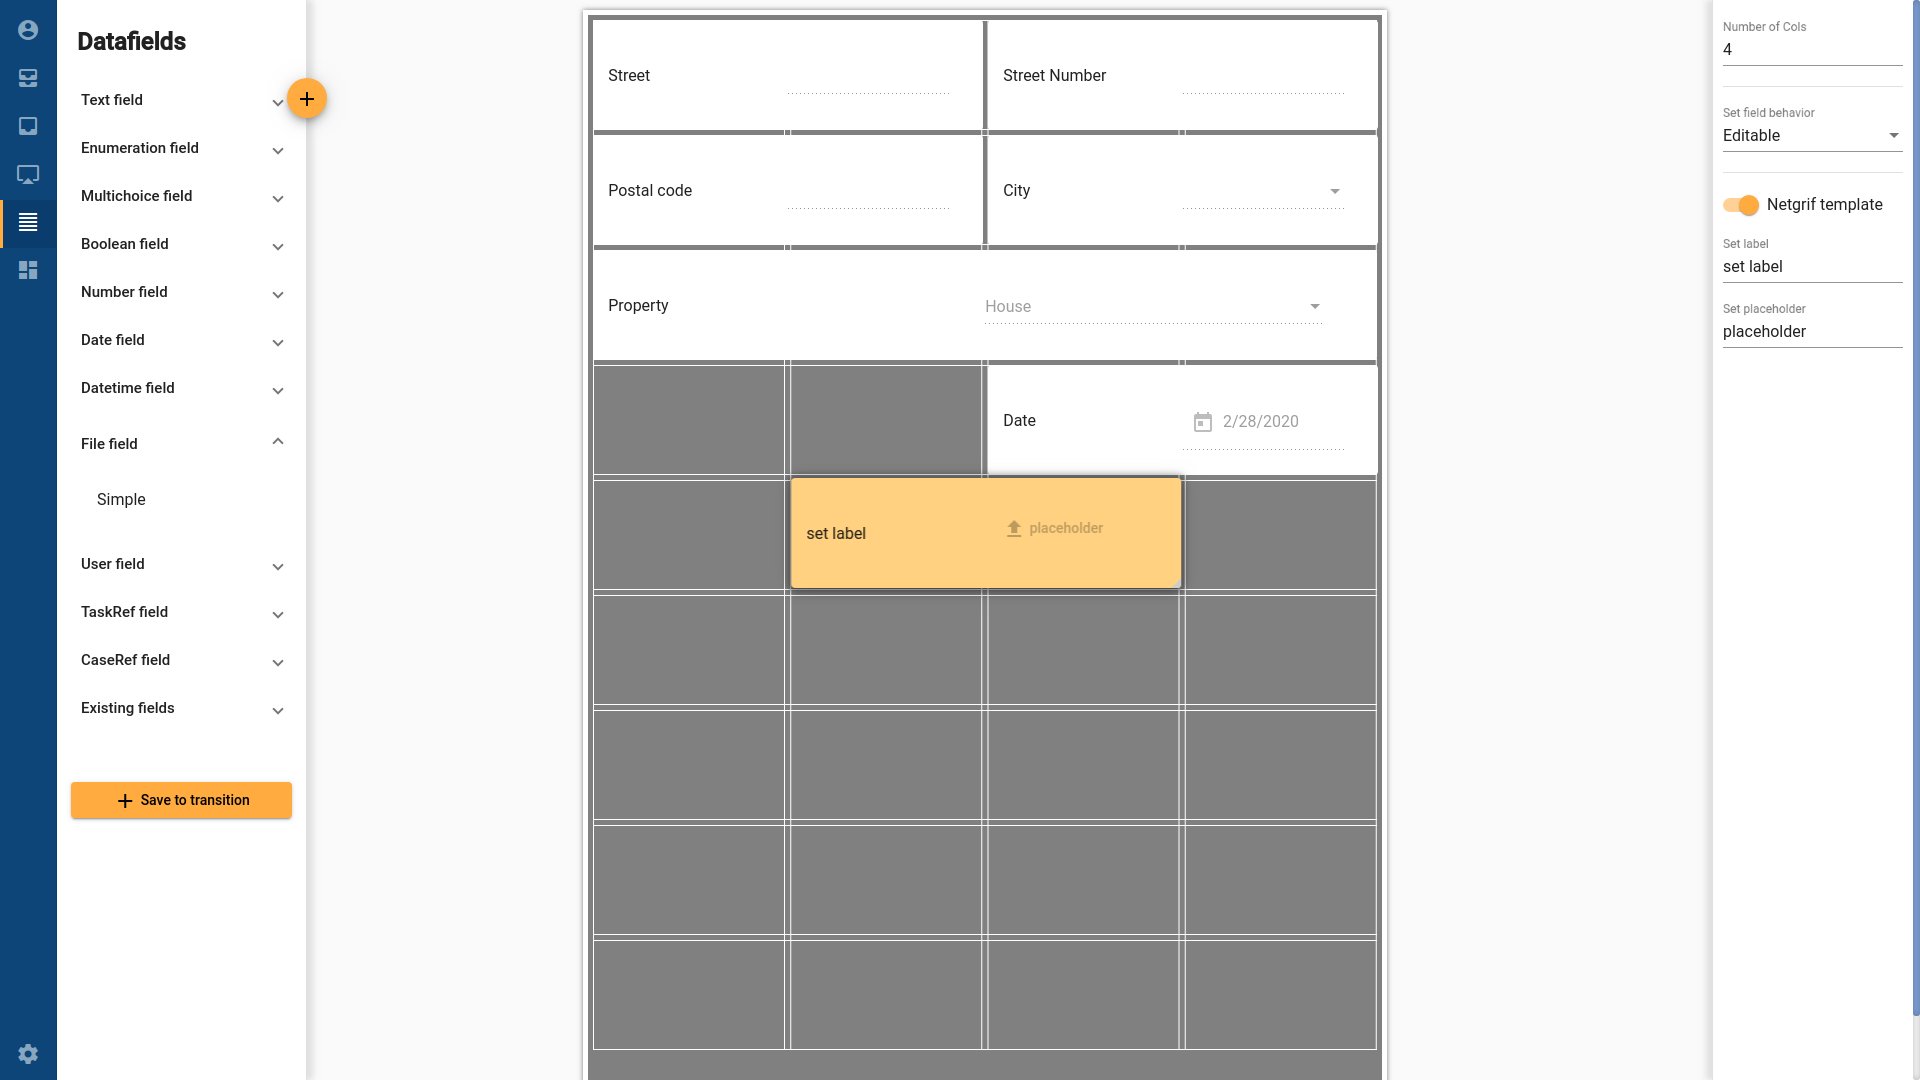
\includegraphics[width=0.9\textwidth]{images/form_view.png}
  \caption{Form builder}
  \label{fig:form_builder}
\end{figure}
